\section{Auswertung}
Zur Auswertung der in diesem Versuch aufgenommenen Daten wird die \textit{Python} 3.8.0 Bibliothek
\textit{Numeric Python} \cite{numpy} genutzt. Ergebnisse werden mit der Bibliothek \textit{matplotlib} \cite{matplotlib} grafisch
dargestellt. Des Weiteren werden die Bibliotheken \textit{uncertainties} \cite{uncertainties} und \textit{SciPy} \cite{scipy} genutzt. Erstere dient zur Automatisierung der Gauß'schen Fehlerfortpflanzung gemäß der Formel
\begin{equation*}
  \Delta y = \sqrt{\sum \left(\frac{\partial y}{\partial x_i}\cdot \Delta x_i \right)^2},
\end{equation*}
wobei $\Delta y$ der Fehler einer aus mehreren fehlerbehafteten Größen $x_i$ zu bestimmenden Größe $y$ ist. $\Delta x_i$ ist hierbei der Fehler der Größe $x_i$. Letztere dient zur Bestimmung der freien Parameter von Ausgleichsfunktionen nach der Methode der kleinsten Quadrate. Die freien Parameter werden also so bestimmt, dass die Summe der quadrierten Abweichungen der Messpunkte von der Ausgleichsfunktion minimal wird.

\newpage
\subsection{Invertierender Linearverstärker}
Zur Untersuchung des invertierenden Linearverstärkers wurden drei Messreihen mit verschiedenen Widerständen im Frequenzbereich $\SIrange{0.01}{1000}{\kilo\hertz}$ aufgenommen. Hierbei wurden jeweils Frequenz $f$, Ausgangsspannung $U_\mathrm{a}$ und zeitliche Differenz $\Delta t$ zwischen den Maxima von Ein- und Ausgangsspannung aufgenommen, welche \autoref{tab:lin_1} bis \ref{tab:lin_3} zu entnehmen sind. Die Widerstandswerte und die sich daraus über \autoref{eqn:verhaeltnis} ergebende theoretische Leerlaufverstärkung sind \autoref{tab:widerstaende} zu entnehmen. Die Eingangsspannung betrug dabei immer $U_\mathrm{e} = \SI{50}{\milli\volt}$.

\begin{table}[H]
  \centering
  \caption{Im Linearverstärker verbaute Widerstände und theoretische Leerlaufverstärkung.}
  \begin{tabular}{c c c c}
    \toprule
    & Messung 1 & Messung 2 & Messung 3\\
    \midrule
    $R_1$/$\si{\kilo\ohm}$ & $\num{1}$ & $\num{1}$ & $\num{15}$\\
    $R_2$/$\si{\kilo\ohm}$ & $\num{100}$ & $\num{150}$ & $\num{100}$\\
    $V_{0,\mathrm{Theo}}$ & $\num{100}$ & $\num{150}$ & $6.\bar{6}$\\
    \bottomrule
  \end{tabular}
  \label{tab:widerstaende}
\end{table}

In \autoref{fig:lin_verstaerkung} sind die aufgenommenen Verstärkungswerte in Abhängigkeit der Frequenz in doppelt logarithmischen Diagrammen für alle Messungen dargestellt.

\begin{figure}[H]
  \centering
  \begin{subfigure}{.65\textwidth}
    \includegraphics[width=\linewidth]{plots/linearverstaerker_1.pdf}
    \subcaption{$R_1 = \SI{1}{\kilo\ohm}$ und $R_2 = \SI{100}{\kilo\ohm}$.}
  \end{subfigure}
  \begin{subfigure}{.65\textwidth}
    \includegraphics[width=\linewidth]{plots/linearverstaerker_2.pdf}
    \subcaption{$R_1 = \SI{1}{\kilo\ohm}$ und $R_2 = \SI{150}{\kilo\ohm}$.}
  \end{subfigure}
  \begin{subfigure}{.65\textwidth}
    \includegraphics[width=\linewidth]{plots/linearverstaerker_3.pdf}
    \subcaption{$R_1 = \SI{15}{\kilo\ohm}$ und $R_2 = \SI{100}{\kilo\ohm}$.}
  \end{subfigure}
  \caption{Verstärkung in Abhängigkeit der Frequenz der Eingangsspannung für die drei Messreihen.}
  \label{fig:lin_verstaerkung}
\end{figure}

Durch das in jedem Plot zu sehende Plateau wird eine konstante Ausgleichsgerade der Form
\begin{equation}
\log_{10} (V) = b
\label{eq:fit_leer}
\end{equation}
gelegt, um die Leerlaufverstärkung des jeweiligen Aufbaus zu ermitteln. Für die drei Messreihen ergeben sich die Werte
\begin{align*}
  b_1 = \num{1.99 \pm 0.012} && b_2 = \num{2.17 \pm 0.009} && b_3 = \num{1.013 \pm 0.009}.
\end{align*}
Die Leerlaufverstärkung lässt sich dann mithilfe von Gleichung \eqref{eq:fit_leer} bestimmen zu $V_0 = 10^{b}$, wodurch sich die Werte
\begin{align*}
  V_{0,1} = \num{97 \pm 2.70} && V_{0,2} = \num{148 \pm 3.20} && V_{0,3} = \num{10.3 \pm 0.22}
\end{align*}
ergeben.

Zur Bestimmung der Grenzfrequenz $f_\mathrm{Grenz}$, welche definiert ist als die Frequenz, bei der $V = \frac{1}{\sqrt{2}}$ gilt, wird durch den abfallenden Bereich der Messungen eine Funktion der Form
\begin{equation}
  \log_{10} (V) = a \cdot \log_{10} (f/\SI{1}{\kilo\hertz}) + c
  \label{eq:fit_lin_abfall}
\end{equation}
gelegt. Die hierbei ermittelten Parameter lauten
\begin{align*}
  a_1 = \num{-0.86 \pm 0.05} && a_2 = \num{-0.98 \pm 0.05} && a_3 = \num{-0.7 \pm 0.11} && \\
  c_1 = \num{2.83 \pm 0.08} && c_2 = \num{3.1 \pm 0.11} && c_3 = \num{2.2 \pm 0.27} && .
\end{align*}
Für die Grenzfrequenz gilt durch Umstellen von Gleichung \eqref{eq:fit_lin_abfall}
\begin{equation*}
  f_\mathrm{Grenz}/\SI{1}{\kilo\hertz} = 10^{\frac{\log \left(\frac{1}{\sqrt{2}}\right) - c}{a}},
\end{equation*}
woraus sich für die drei Messreihen die Werte
\begin{align*}
  f_{\mathrm{Grenz},1} = \SI{3.1 \pm 1.5 e3}{\kilo\hertz} && f_{\mathrm{Grenz},2} = \SI{2.1 \pm 1.0 e3}{\kilo\hertz} && f_{\mathrm{Grenz},3} = \SI{3.0 \pm 5.0 e3}{\kilo\hertz}
\end{align*}
ergeben.
Für das Bandbreitenprodukt ergeben sich hiermit die Werte
\begin{align*}
  B_1 = \num{300758 \pm 146429} && B_2 = \num{312873 \pm 150069} && B_3 = \num{32884 \pm 52863}.
\end{align*}

% Operationsverstärker bestehen im Allgemeinen aus mindestens drei Verstärkerstufen. Deren Kollektorwiderstände bilden mit der Eingangskapazität der folgenden Stufen RC-Glieder, die als Tiefpässe wirken und eine Phasenverschiebung bewirken. Hierdurch wird die Verstärkung des Operationsverstärkers bei hohen Frequenzen gedämpft.
Im Allgemeinen weisen Operationsverstärker eine frequenzabhängige Phasenverschiebung auf, welche bei großen Frequenzen für eine abschwächende Verstärkung durch Interferenz sorgt. Dieses Verhalten soll nun untersucht werden.

Die Phasenverschiebung zwischen Ein- und Ausgangsspannung wird berechnet über $\Delta \phi = 2 \pi f \cdot \Delta t$ und ist in Abhängigkeit der Frequenz für alle drei Messreihen in \autoref{fig:phase} aufgetragen.

\begin{figure}[H]
  \centering
  \begin{subfigure}{.65\textwidth}
    \includegraphics[width=\linewidth]{plots/linearverstaerker_phase_1.pdf}
    \subcaption{$R_1 = \SI{1}{\kilo\ohm}$ und $R_2 = \SI{100}{\kilo\ohm}$.}
  \end{subfigure}
  \begin{subfigure}{.65\textwidth}
    \includegraphics[width=\linewidth]{plots/linearverstaerker_phase_2.pdf}
    \subcaption{$R_1 = \SI{1}{\kilo\ohm}$ und $R_2 = \SI{150}{\kilo\ohm}$.}
  \end{subfigure}
  \begin{subfigure}{.65\textwidth}
    \includegraphics[width=\linewidth]{plots/linearverstaerker_phase_3.pdf}
    \subcaption{$R_1 = \SI{15}{\kilo\ohm}$ und $R_2 = \SI{100}{\kilo\ohm}$.}
  \end{subfigure}
  \caption{Phasenverschiebung zwischen Ein- und Ausgangsspannung als Funktion der Frequenz der Eingangsspannung.}
  \label{fig:phase}
\end{figure}
Die Phasenverschiebung $\pi$ bei niedrigen Frequenzen ist Folge der invertierenden Eigenschaft des Linearverstärkers und somit erwartet. Da die Verstärkung bei hohen Frequenzen abnimmt, ist mit einer ansteigenden Phasenverschiebung zu rechnen, allerdings sollte diese gegen $\frac{3\pi}{2}$ laufen, da in diesem Fall Eingangs- und Ausgangsspannung destruktiv interferieren würden. Stattdessen läuft die Phasenverschiebung bei hohen Frequenzen in allen Messreihen gegen $2\pi$.

\subsection{Umkehr-Integrator}
Zur Untersuchung des Integrators wurde die Ausgangsspannung $U_\mathrm{a}$ in Abhängigkeit der Frequenz $f$ der Eingangsspannung aufgenommen, wobei es sich bei letzterer um ein sinusförmiges Signal handelt. Hierbei wurden ein Widerstand mit $R = \SI{10}{\kilo\ohm}$ und ein Kondensator mit Kapazität $C = \SI{100}{\nano\farad}$ verwendet. Die Messwerte sind \autoref{tab:int} im \autoref{sec:anhang} zu entnehmen und grafisch in \autoref{fig:int_messung} dargestellt.

\begin{figure}[H]
  \centering
  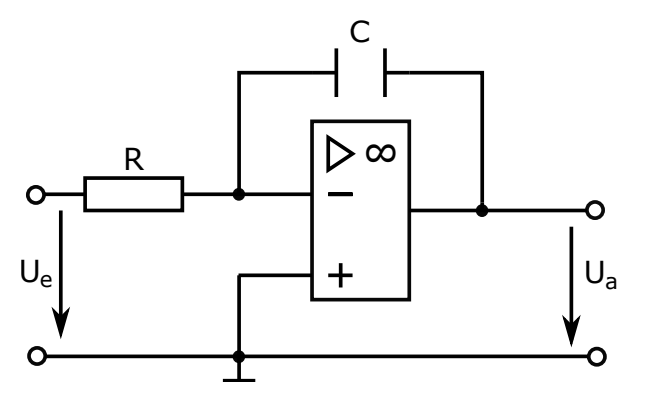
\includegraphics[width=.65\textwidth]{plots/integrator.pdf}
  \caption{Ausgangsspannung als Funktion der Frequenz an einem Umkehr-Integrator.}
  \label{fig:int_messung}
\end{figure}
Da es sich um einen doppelt-logarithmisches Diagramm handelt, wird der erwartete Zusammenhang zwischen Ein-und Ausgangsspannung zu
\begin{equation*}
  \log_{10} (U_\mathrm{a}/\SI{1}{\volt}) = \log_{10} (- \frac{U_\mathrm{e}}{2\pi R C}/\SI{1}{\volt\per\milli\second}) - \log_{10} (f/\SI{1}{\kilo\hertz}).
\end{equation*}
Zur Überprüfung dieses Zusammenhangs wird durch die aufgenommenen Werte eine Ausgleichsgerade der Form
\begin{equation}
  \log_{10} (U_\mathrm{a}/\SI{1}{\volt}) = a \cdot \log_{10} (f/\SI{1}{\kilo\hertz}) + b
  \label{eq:fit_int}
\end{equation}
gelegt. Die hierbei erhaltenen Fit-Parameter lauten
\begin{align*}
  a = \num{-1.095 \pm 0.023} && b = \num{-1.560 \pm 0.034}.
\end{align*}
Im Vergleich mit dem erwarteten Zusammenhang lässt sich feststellen, dass $a$ nicht exakt $-1$ beträgt, der Verlauf allerdings in guter Näherung reproduziert werden konnte.

Weiterhin wurde die integrierende Eigenschaft des Integrators anhand eines Dreieck-, Rechteck- und eines Sinus-Signals untersucht. Die dazugehörigen Signale sind \autoref{fig:int_oszi} zu entnehmen, wobei Channel 1 (CH1) das jeweilige Ausgangs- und Channel 2 (CH2) das jeweilige Eingangssignal zeigt.

\begin{figure}[H]
  \centering
  \begin{subfigure}{.4\textwidth}
    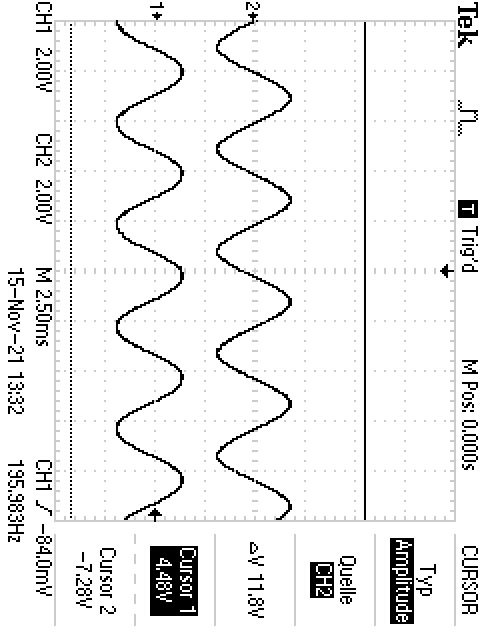
\includegraphics[width=\linewidth]{data/ALL0059/F0059TEK.JPG}
    \subcaption{Ein- und Ausgangsspannung des Umkehr-Integrators mit Sinus-Spannung als Eingangsspannung.}
  \end{subfigure}
  \begin{subfigure}{.4\textwidth}
    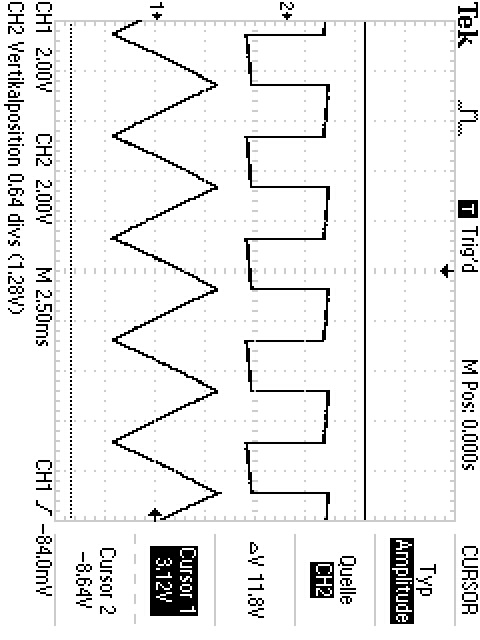
\includegraphics[width=\linewidth]{data/ALL0060/F0060TEK.JPG}
    \subcaption{Ein- und Ausgangsspannung des Umkehr-Integrators mit  Rechteck-Spannung als Eingangsspannung.}
  \end{subfigure}
  \begin{subfigure}{.4\textwidth}
    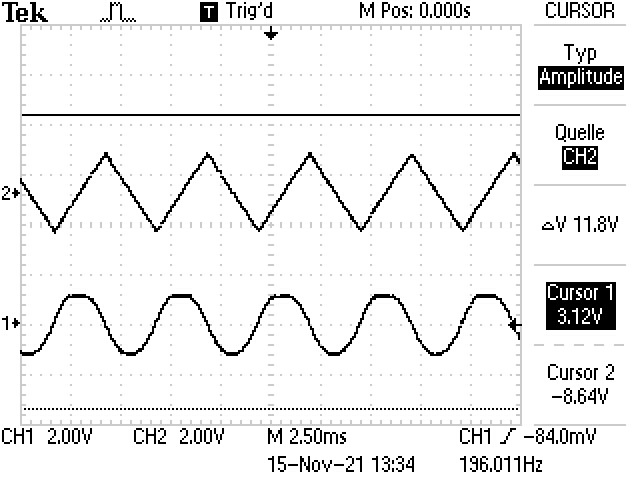
\includegraphics[width=\linewidth]{data/ALL0061/F0061TEK.JPG}
    \subcaption{Ein- und Ausgangsspannung des Umkehr-Integrators mit Dreieck-Spannung als Eingangsspannung.}
  \end{subfigure}
  \caption{Ein- und Ausgangssignale der Umkehr-Integrator-Schaltung nach \autoref{fig:umkehrint}  für verschiedene Eingangsspannungen. Die Eingangssignale sind jeweils in Channel 1 (CH1) und die Ausgangssignale in Channel 2 (CH2) zu sehen.}
  \label{fig:int_oszi}
\end{figure}

Das Integral einer Rechteck-Spannung ist eine Dreieck-Spannung, das Integral der Dreieck-Spannung ist eine Parabel und das Integral einer Sinus-Funktion ein Cosinus. All diese Integrale sind auch auf dem Oszilloskop zu sehen. Die integrierende Funktion des Integrators konnte also bestätigt werden.

\newpage
\subsection{Invertierender Differenzierer}
Zur Untersuchung des invertierenden Differenzierers wird analog zum vorherigen Abschnitt vorgegangen. Dabei wurden ein Widerstand mit $R = \SI{100}{\kilo\ohm}$ und ein Kondensator mit Kapazität $C = \SI{22}{\nano\farad}$ verwendet. Die aufgenommenen Messwerte sind \autoref{tab:diff} im \autoref{sec:anhang} zu entnehmen und grafisch in \autoref{fig:diff_messung} dargestellt.

\begin{figure}[H]
  \centering
  \includegraphics[width=.65\textwidth]{plots/differenzierer.pdf}
  \caption{Ausgangsspannung als Funktion der Frequenz bei einem Differenzierer.}
  \label{fig:diff_messung}
\end{figure}

Da es sich um einen doppelt-logarithmischen Plot handelt, wird aus dem Zusammenhang zwischen Ein- und Ausgangsspannung bei einem Sinus-Signal
\begin{equation*}
  \log_{10} (U_\mathrm{a}/\SI{1}{\volt}) = \log_{10} (f/\SI{1}{\kilo\hertz}) + \log_{10} (- 2 \pi R C U_\mathrm{e}/\SI{1}{\volt\micro\second}).
\end{equation*}
Zur Überprüfung dieses Zusammenhangs wird analog zum Integrator eine Ausgleichsgerade nach Gleichung \eqref{eq:fit_int} durch die Messwerte gelegt, wobei sich die Parameter
\begin{align*}
  a = \num{1.002 \pm 0.003} && b = \num{2.838 \pm 0.005}
\end{align*}
ergeben. Folglich lässt sich der theoretische Zusammenhang zwischen Ausgangsspannung und Frequenz experimentell bestätigen.

Weiterhin wurden zur Überprüfung der differenzierenden Eigenschaft des invertierenden Differenzierers Ein- und Ausgangssignale am Oszilloskop untersucht. Die aufgenommenen Bilder sind \autoref{fig:diff_oszi} zu entnehmen.

\begin{figure}[H]
  \centering
  \begin{subfigure}{.496\textwidth}
    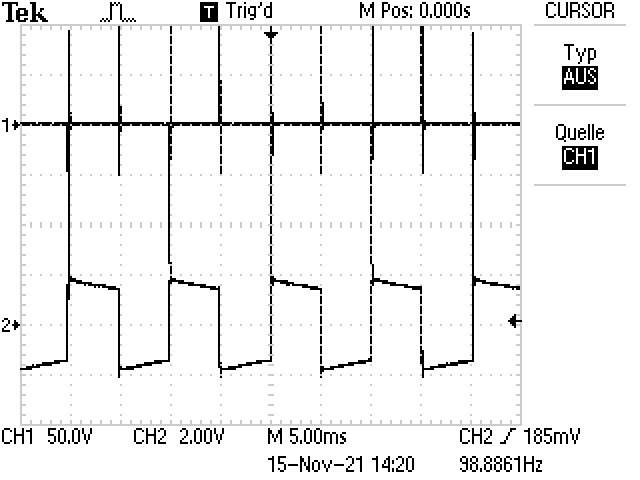
\includegraphics[width=\linewidth]{data/ALL0062/F0062TEK.JPG}
    \subcaption{Ein- und Ausgangsspannung des Umkehr-Differenzierers mit Rechteck-Spannung als Eingangsspannung.}
  \end{subfigure}
  \begin{subfigure}{.496\textwidth}
    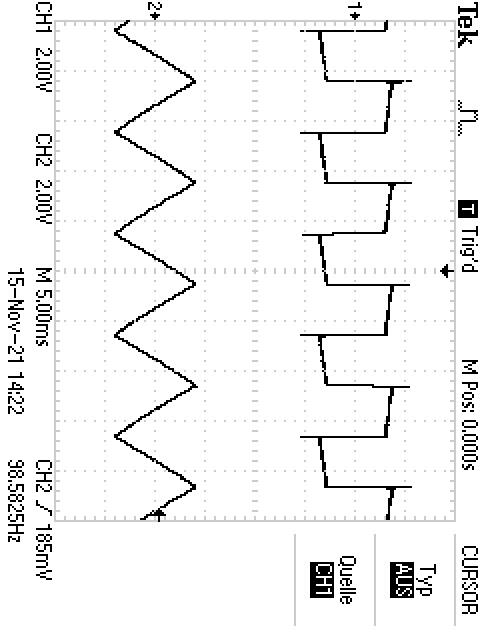
\includegraphics[width=\linewidth]{data/ALL0063/F0063TEK.JPG}
    \subcaption{Ein- und Ausgangsspannung des Umkehr-Differenzierers mit Dreieck-Spannung als Eingangsspannung.}
  \end{subfigure}
  \begin{subfigure}{.496\textwidth}
    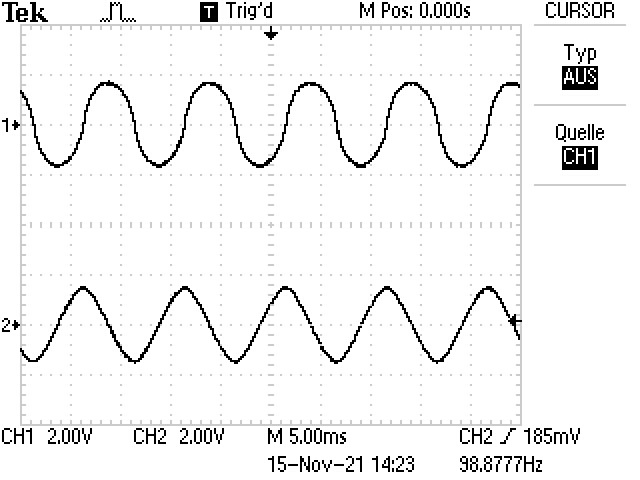
\includegraphics[width=\linewidth]{data/ALL0064/F0064TEK.JPG}
    \subcaption{Ein- und Ausgangsspannung des Umkehr-Differenzierers mit Sinus-Spannung als Eingangsspannung.}
  \end{subfigure}
  \caption{Ein- und Ausgangsspannung einer Umkehr-Differenzierer-Schaltung nach \autoref{fig:umkehrdiff} für Dreieck-, Rechteck- und Sinus-Eingangssignale. Die Eingangssignale sind jeweils in CH2 und die Ausgangssignale in CH1 zu sehen.}
  \label{fig:diff_oszi}
\end{figure}


Bei einer Dreieck-Spannung als Eingangsspannung wird eine Rechteck-Spannung als Ausgangsspannung erwartet, bei einer Rechteck-Spannung als Eingangsspannung werden Peaks einer Delta-Distribution an Stelle der Spannungsänderung erwartet, da diese näherungsweise als Gerade mit unendlicher Steigung zu einem infinitesimalen Zeitpunkt betrachtet werden kann, und bei einem Sinus-Eingangssignal wird als Ausgang ein Cosinus erwartet. Die jeweils erwarteten Ausgangssignale, also jeweils die Ableitung des Eingangssignals, konnten beobachtet und folglich die Funktion des Umker-Differenzierers bestätigt werden, wobei an den Unstetigkeiten des Dreieck-Signals als Eingangssignal das Gibb'sche Phänomen im Ausgangssignal zu beobachten ist. Dieses beschreibt das Auftreten von Über- und Unterschwingungen an den Sprungstellen der Fourierreihen von stückweise stetigen, differenzierbaren Funktionen auftritt und ist in der Elektronik von Bedeutung, da keine reinen Signale erzeugt werden können, sondern nur Approximationen.

\subsection{Nicht-invertierender Schmitt-Trigger}

\begin{figure}[H]
  \centering
  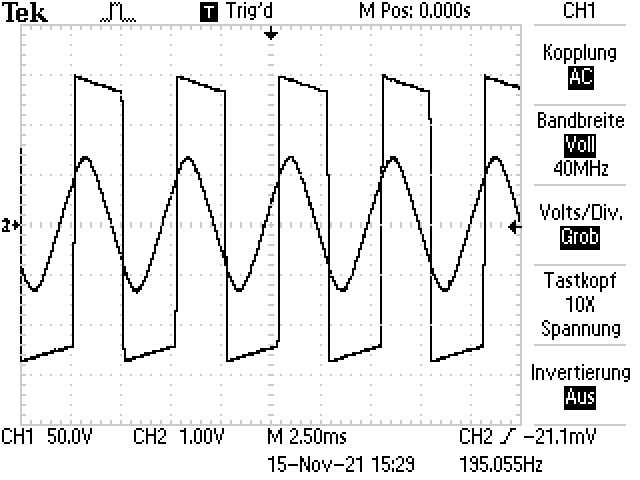
\includegraphics{data/ALL0066/F0066TEK.JPG}
  \caption{Oszilloskop-Bild des Schmitt-Triggers. CH2 zeigt das sinusförmige Eingangssignal. CH1 zeigt ein rechteckförmiges Ausgangssignal.}
  \label{fig:schmitt_oszi}
\end{figure}

Zur Untersuchung des Nicht-invertierenden Schmitt-Triggers werden die Widerstände $R_1 = \SI{10}{\kilo\ohm}$ und $R_2 = \SI{220}{\kilo\ohm}$ verbaut. In \autoref{fig:schmitt_oszi} ist der Verlauf der Ein- und Ausgangsspannung am Oszilloskop dargestellt. Zu sehen ist das sinusförmige Eingangssignal in CH2 und ich CH1 ist das erhaltene rechteckförmige Ausgangssignal zu sehen, auch wenn dieses eine leichte Spannungsabnahme im theoretisch konstanten Bereich aufweist. Dies beeinträchtigt die Funktion des Schmitt-Triggers im Rahmen dieses Versuchs allerdings nicht. Die Vorzeichenwechsel der Ausgangsspannung erfolgt hierbei immer kurz bevor die Eingangsspannung einen Extremalwert erreicht. Dieser Wert kennzeichnet die Kipp-Spannung der Schaltung. Durch Variation der Amplitude der Eingangsspannung kann die Kipp-Spannung bestimmt werden, indem die Amplitude ermittelt wird, bei der das Ausgangssignal zum rechteckförmigen Signal wird. Die Kipp-Spannung wurde bei $U_{\mathrm{e, Kipp}} = \SI{680}{\milli\volt}$ gefunden. Der theoretische Wert beträgt $U_{S_{\pm}} = 0.6\bar{81} \, \si{\volt}$.

\newpage
\subsection{Signalgenerator}
In \autoref{fig:signalgenerator_oszi} ist der Spannungsverlauf der Eingangsspannung und der Ausgangsspannung an einem Signalgenerator zu sehen.

\begin{figure}[H]
  \centering
  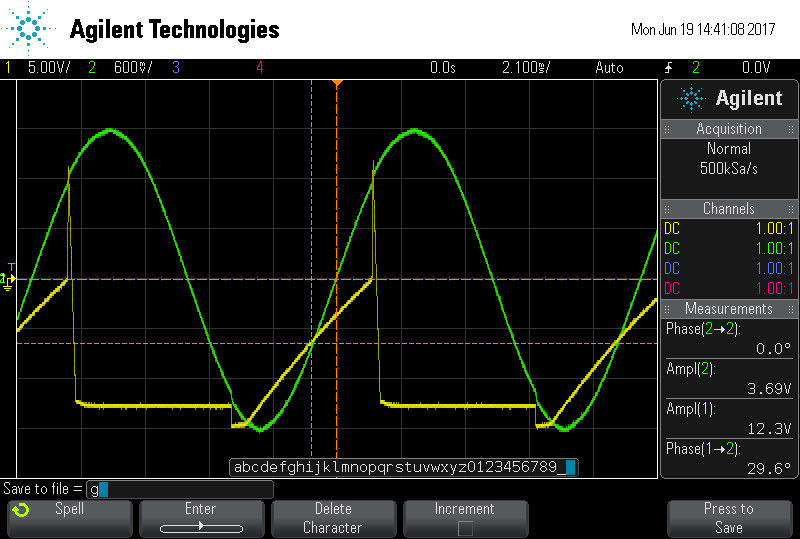
\includegraphics[width=\textwidth]{signalgen.png}
  \caption{Ein- (grün) und Ausgangssignal (gelb) an einem Signalgenerator\cite{ahlmann_2021}.}
  \label{fig:signalgenerator_oszi}
\end{figure}
Am aufsteigenden Ast der Ausgangsspannung ist wie zu erwarten ein Dreieck-Signal zu erkennen. Der abfallende Ast hingegen besteht vor Allem aus Unstetigkeiten und einem Rechteck-Signal. Hier versagt folglich der Integrator. Trotzdem kann die Frequenz des Ausgangssignals bestimmt werden. Das Oszilloskopbild ist $640$ Pixel breit und deckt eine Zeitspanne von $10 \cdot \SI{2.1}{\milli\second} = \SI{21}{\milli\second}$ ab. Folglich gilt für die Zeit pro Pixel $t_\mathrm{Pixel} \approx \SI{0.0328}{\milli\second}$. Der Abstand der zwei zu sehenden Minima der Ausgangsspannung beträgt $304$ Pixel. Für die Periodendauer $T$ der Ausgangsspannung gilt folglich

\begin{equation*}
  T = 304 \cdot t_\mathrm{Pixel} = \SI{9.975}{\milli\second}
\end{equation*}
und über den Zusammenhang $T = f^{-1}$ gilt demnach für die Frequenz
\begin{equation*}
  f = \SI{100.25}{\hertz}.
\end{equation*}
Für das Verhältnis der Bauteilgrößen muss nach Gleichung \eqref{eq:dreieck} also
\begin{equation*}
  \frac{R_2}{C R_1 R_3} = \SI{25.063}{\hertz}
\end{equation*}
gelten. Mit den vorher verwendeten Bauteilen lässt sich dieser Wert ungefähr erreichen, wenn der Kondensator mit Kapazität $C = \SI{22}{\nano\farad}$ und die Widerstände $R_1 = \SI{10}{\kilo\ohm}$, $R_2 = \SI{1}{\kilo\ohm}$ und $R_3 = \SI{100}{\kilo\ohm}$ verwendet werden. Mit einem Kondensator der Kapazität $C = \SI{25}{\nano\farad}$ wäre der Wert bei gleichen Widerständen noch besser zu erreichen.
Es können aber auch $R_1$ und $R_2$ bzw. $R_2$ und $R_3$ beliebig ausgetauscht werden, solange das Verhältnis der beiden Widerstände beibehalten wird und die anderen Bauteile beibehalten werden.
